% Figure 1 composite — vertical narrative with unified d/e/f module.
\pdfminorversion=7
\documentclass{article}
\usepackage[paperwidth=183mm,paperheight=252mm,margin=2.5mm]{geometry}
\usepackage{graphicx}
\usepackage{tikz}
\pagestyle{empty}
\setlength{\parindent}{0pt}

\begin{document}
\begin{tikzpicture}[remember picture, overlay,
                    every node/.style={anchor=north west, inner sep=0pt}]

  % ===================== ROW 1 : global signal + selection ====================
  % a, b1, c share one top narrative row
  \node at (3mm,   -4mm)  {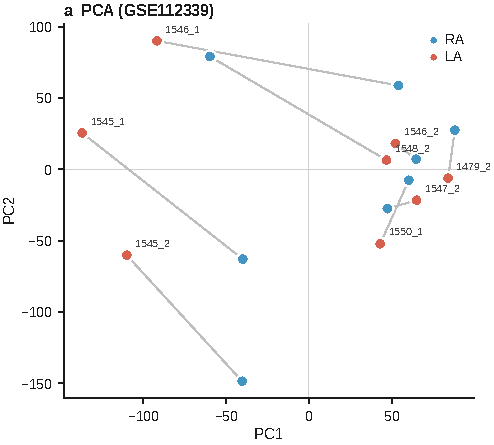
\includegraphics[width=43mm]{fig1a_pca_la_vs_ra.pdf}};
  \node at (49mm,  -4mm)  {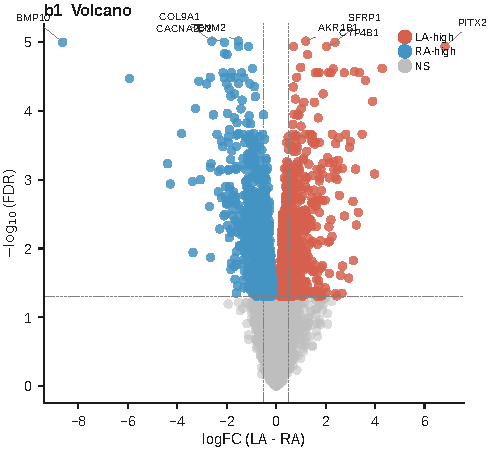
\includegraphics[width=43mm]{fig1b_volcano.pdf}};
  \node at (95mm,  -4mm)  {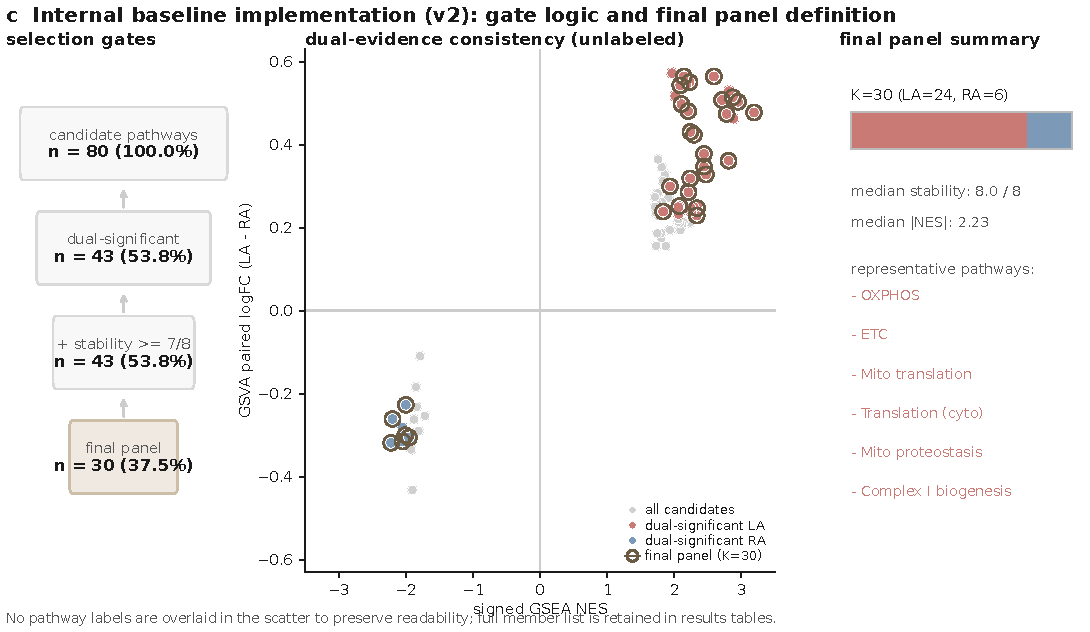
\includegraphics[width=85mm]{fig1c_dual_method_selection.pdf}};

  % ===================== ROW 2 : baseline module (part I) =====================
  \node[anchor=west] at (3mm, -49mm) {\fontsize{9}{10}\selectfont \textbf{Baseline module (shared 30-program row system): d / e / f}};
  \node at (7mm, -56mm) {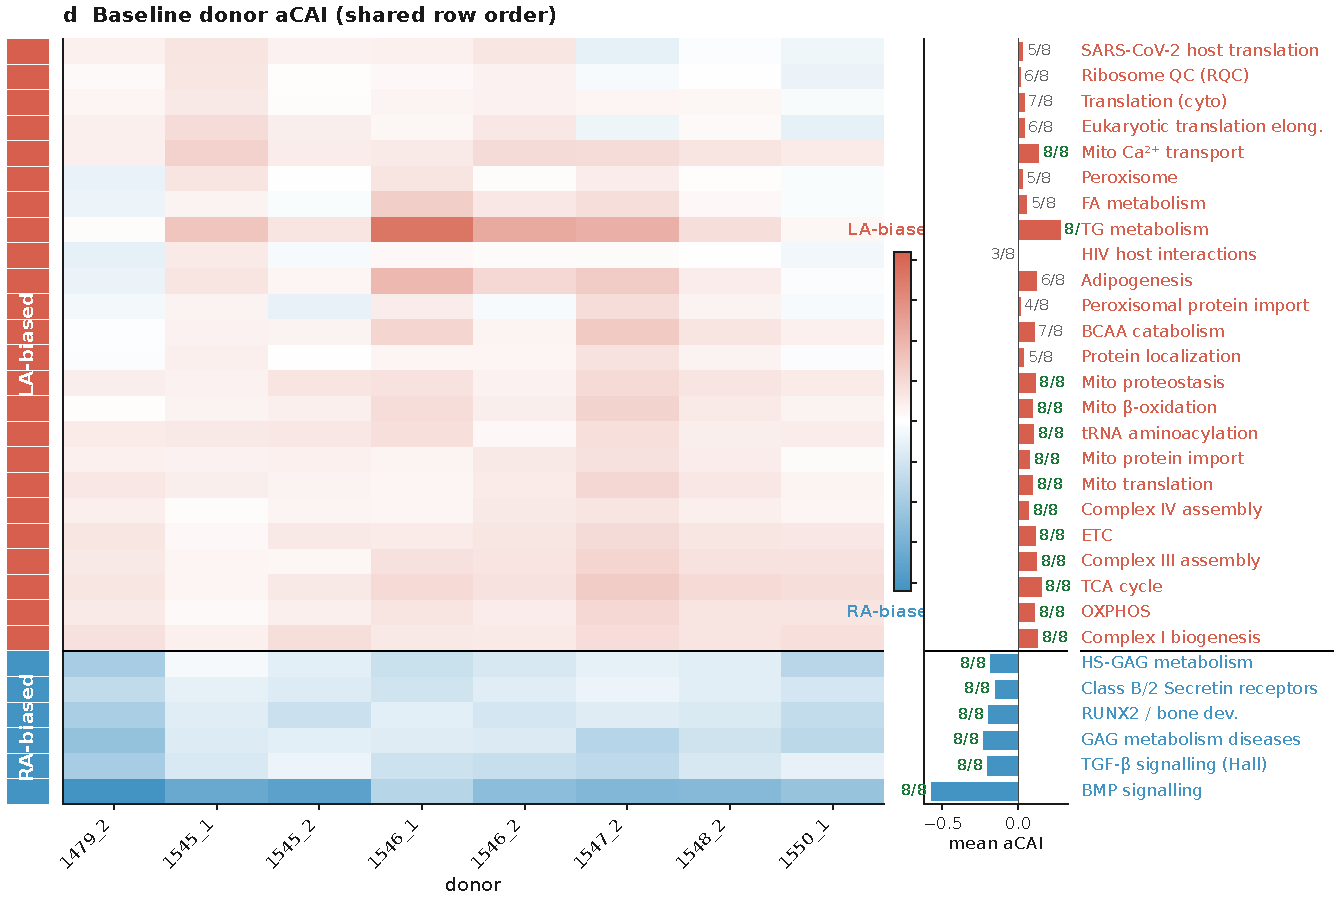
\includegraphics[width=84mm]{fig1d_baseline_donor_aCAI.pdf}};
  \node at (92mm, -56mm) {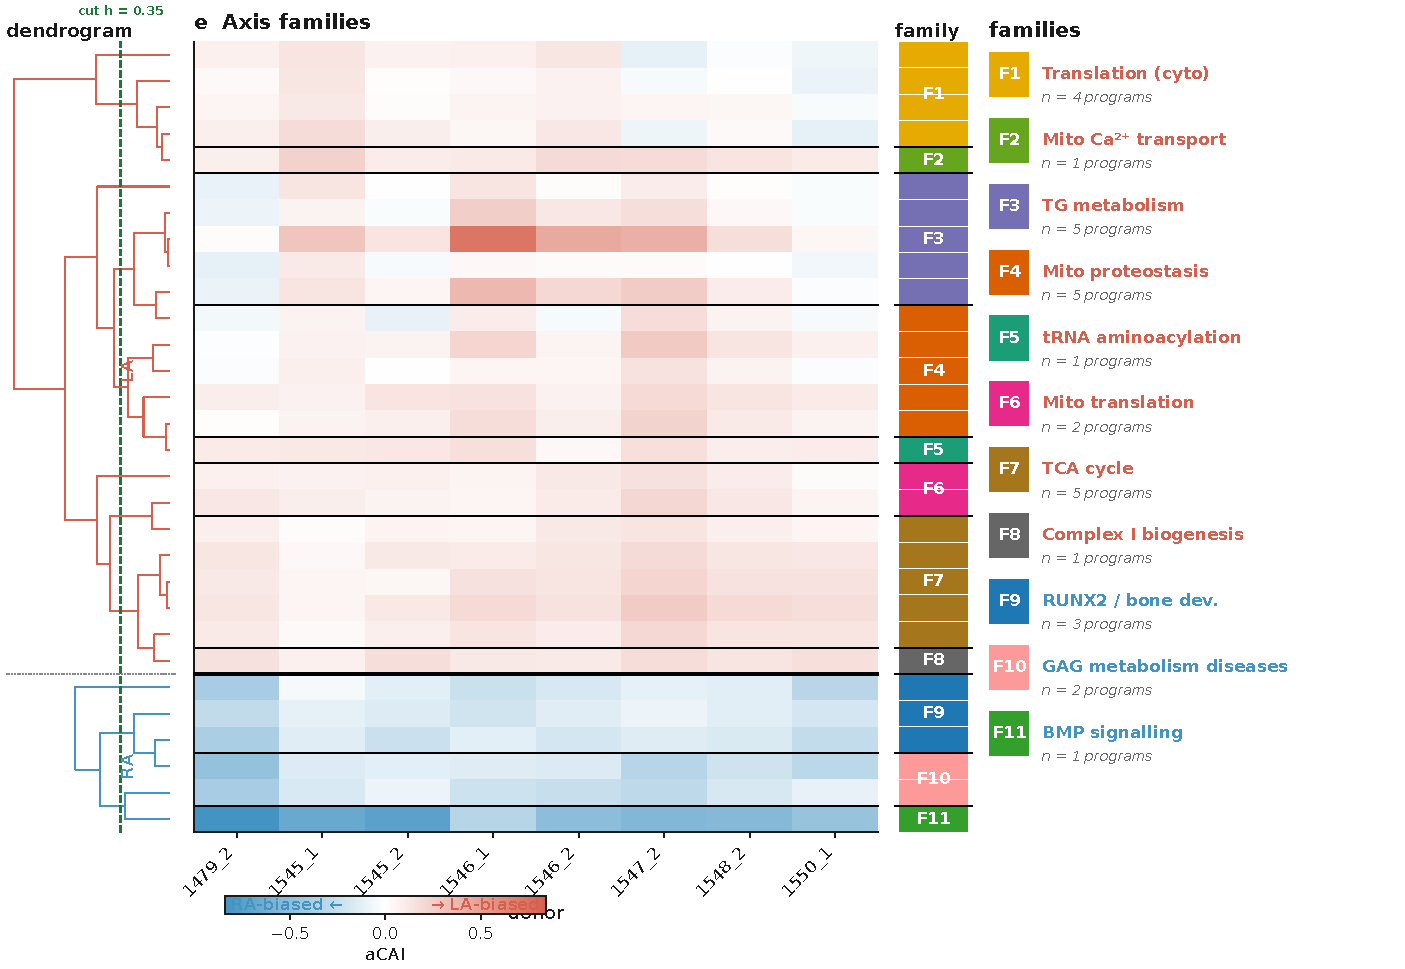
\includegraphics[width=84mm]{fig1e_baseline_axis_families.pdf}};

  % ===================== ROW 3 : baseline module (part II) ====================
  \node at (15mm, -122mm) {\includegraphics[width=154mm]{fig1f_baseline_attribution.pdf}};

\end{tikzpicture}
\end{document}
